\documentclass{amsart}
\usepackage{tikz}
\title{Problem Set 3 Solutions}
\begin{document}
\maketitle

\section*{Part A (9 marks)} 
State Euler's Theorem for plane graphs, and use it to show that if a $G$ is a plane graph with no vertices of degree less than 3 or cycles with length less than 4, then $G$ must have at least 8 vertices and at least 12 edges.  Give an example to show that these bounds cannot be improved.

\begin{proof}
  Euler's Theorem for plane graphs states that if $G$ is drawn on the sphere so that no edges cross, and the $G$ has $v$ vertices and $e$ edges, and in the drawing there are $f$ faces, then
  $$v-e+f=2$$

To prove the bound, we combine Euler's Theorem with handshaking theorems.
Handshaking between vertices and edges, together with the fact that every vertex has degree at least 3 gives:
$$2e=\sum_{v} d(v)\geq 3v$$
and so $v\leq 2e/3$

Similarly, Handshaking between faces and edges, together with the fact that every cycle (and hence every face) has degree at least 4 gives
$$2e=\sum_{f} d(f)\geq 4f$$
and so $f\leq e/2$.

Substituting these inequalities into Euler's formula gives:
$$2=v-e+f\leq 2e/3-e+e/2=e/6$$
and hence $e\geq 12$ as desired.

The inequality we currently have for $v$ points the wrong way; instead we go back to Euler's formula, and first substitute our inequality for $f$, and then our inequality for $e$:

\begin{align*}
  2&=v-e+f \\
  &\leq v-e+e/2 =v-e/2\\
  &\leq v-12/2
\end{align*}

and so $v\geq 8$ as desired.

The cube graph is planar, has no cycles of length less than 4, and every vertex has degree 3, so it satisfies the hypotheses of our bound; furthermore, it has 8 verties and 12 edges, and so we see our bounds are tight.
\end{proof}

\section*{Part B (2 Marks)}
Suppose that $G$ is any graph with no vertices of degree less than 3 or cycles with length less than 4 -- must $G$ be planar?  Justify your answer.

\begin{proof}
  No, $G$ need not be planar: $K_{3,3}$ is a counter example.  Every vertex has degree 3, there are no loops, multiple edges, or triangles, so every cycle has length at least 4, and $K_{3,3}$ isn't planar.
  \end{proof}


The rest of this question use the graph $\Gamma$ show below.
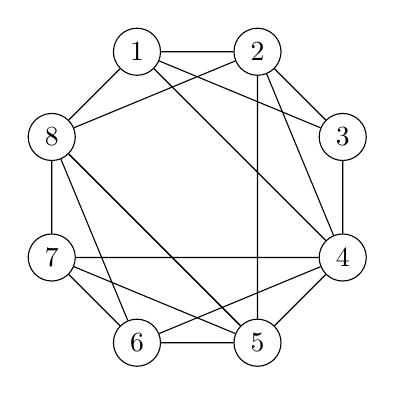
\begin{tikzpicture}
\tikzstyle{vertex}=[circle, draw, minimum size=17pt, inner sep=0pt]

\foreach \x in {1,2,...,8} {
\node[vertex] (\x) at (157.5-\x*45:2cm) {\x};
}  
\draw (1)--(2)--(3)--(4)--(5)--(6)--(7)--(8)--(1)--(3);
\draw (5)--(7)--(4);

\draw (5)--(8)--(2);
\draw (4)--(6)--(8)--(5)--(2)--(4)--(1);
\end{tikzpicture}


\section*{Part C (5 Marks)}

Use the Planarity Algorithm for Hamiltonian Graphs (with the Hamiltonian cycle 123456781) to show that $\Gamma$ is not planar.

\begin{proof}
  We find the crossing graph is as follows:
\begin{center}
  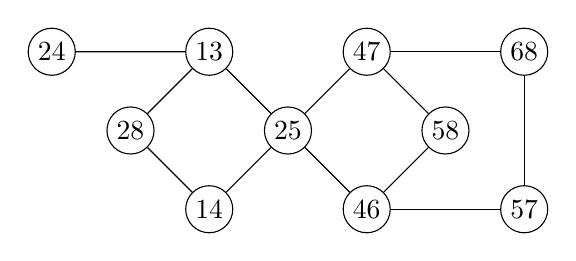
\begin{tikzpicture}
    \tikzstyle{vertex}=[circle, draw, minimum size=17pt, inner sep=0pt]
    \node[vertex] (bd) at (0,2) {24};
    \node[vertex] (ac) at (2,2) {13};
    \node[vertex] (bh) at (1,1) {28};
    \node[vertex] (ad) at (2,0) {14};
    \node[vertex] (be) at (3,1) {25};
    \node[vertex] (gd) at (4,2) {47};
    \node[vertex] (df) at (4,0) {46};
    \node[vertex] (he) at (5,1) {58};
    \node[vertex] (hf) at (6,2) {68};
    \node[vertex] (ge) at (6,0) {57};
    \draw (bd)--(ac)--(bh)--(ad)--(be)--(ac);
    \draw (be)--(gd)--(he)--(df)--(be);
    \draw (gd)--(hf)--(ge)--(df);
  


    \end{tikzpicture}
\end{center}
This crossing graph is not bipartite as it has the five cycle 25,47,68,57,46,25.  Hence, $\Gamma$ is not planar.
\end{proof}


\subsection*{Part D (5 Marks)}

State Kuratowski's Theorem, and use it to give another proof that $\Gamma$ isn't planar.

\begin{proof}
  Kuratowski's theorem states that a graph $G$ is planar if and only if $G$ does not have a subgraph that is a subdivision of $K_5$ or $K_{3,3}$.

 The graph $\Gamma$ shown has subdivisions of both $K_5$ and $K_{3,3}$.

For instance, to find a $K_5$, take as our vertices 4,5,6,7,8.  $\Gamma$ contains all edges between these vertices except the edge between 4 and 8, but we can connect these through 1, for instance.  

An example of a $K_{3,3}$ is to take 2,6,7 as our red vertices, and 4,5 and 8 as our blue vertices, then already every red vertex is adjacent to every blue vertex and we don't even need to subdivide the $K_{3,3}$.

Only one such subgraph was necessary, and there are undoubtedly others; after exhibiting such a subgraph, you should say, and ``and so by Kuratowski's theorem $\Gamma$ is not planar''.

  \end{proof}

\subsection*{Part E (4 Marks)}


Draw $\Gamma$ on the torus so that no edges cross.

\begin{proof}
The work done to find the crossing graph can help with this: we see that the graph was almost planar, with really only one 5 cycle as a problem.  If we draw both 47 and 68 outside (which we can do without having them cross, thanks to the identifications of the edges of the square), then we've broken up that 5 cycle, and we can draw 24, 28, 25, 58, and 57 inside the octagon with no crossings, and draw the remaining edges outside, for example, like this:

\begin{center}
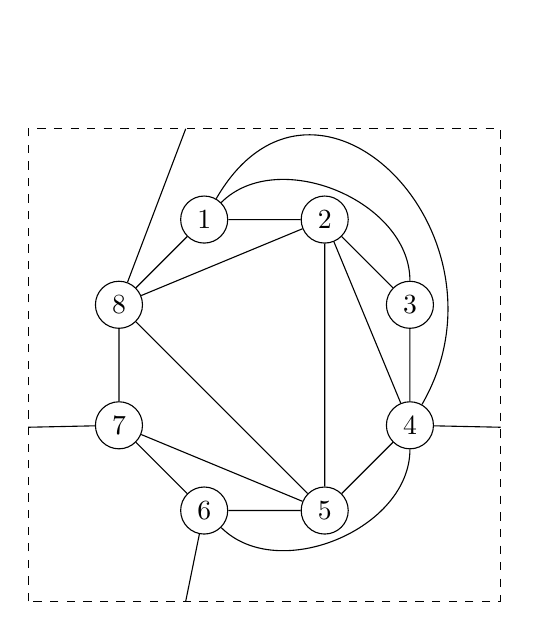
\begin{tikzpicture}
\tikzstyle{vertex}=[circle, draw, minimum size=17pt, inner sep=0pt]

\foreach \x in {1,2,...,8} {
\node[vertex] (\x) at (157.5-\x*45:2cm) {\x};
}  
\draw (1)--(2)--(3)--(4)--(5)--(6)--(7)--(8)--(1);
\draw (4)--(2)--(8)--(5)--(2);
\draw (5)--(7);

\draw (3) to [out=90, in=45] (1);
\draw (1) to [out=60, in=60, distance=2.5cm] (4);
\draw (4) to [out=-90, in=-45] (6);
\draw (4) to (3, -.79);
\draw (-3, -.79) to (7);
\draw (8) to (-1,3);
\draw (-1,-3) to (6);

\draw[dashed] (-3,-3) rectangle (3,3);

\end{tikzpicture}
\end{center}
Other drawings are possible, of course.
  \end{proof}


\end{document}
